\documentclass[french]{article}
\usepackage[T1]{fontenc}
\usepackage[utf8]{inputenc}
\usepackage[french]{babel}
\usepackage{amsmath}
\usepackage{mathtools}
\usepackage{color}
\usepackage[svgnames,dvipsnames]{xcolor} 
\usepackage{soul}
\usepackage{amssymb}
\usepackage{enumitem}
\usepackage{multicol}
\usepackage[left=2cm,right=2cm,top=2cm,bottom=2cm]{geometry}
\newcommand{\mathcolorbox}[2]{\colorbox{#1}{$\displaystyle #2$}}
\usepackage{pifont}
\usepackage{pst-all}
\usepackage{pstricks}
\usepackage{delarray}
\usepackage{setspace}
\usepackage{graphicx}
\usepackage{hyperref}
\usepackage{nicematrix}
\usepackage{listings}
\usepackage{float}

\hypersetup{
	colorlinks=true,
	linkcolor=blue,
	filecolor=magenta,      
	urlcolor=cyan,
	pdfpagemode=FullScreen,
}

\usepackage{amsthm}
\newtheorem*{Rem}{Remarque}

\newenvironment{conclusion}[1]{%
	\begin{center}\normalfont\textbf{Conclusion}\end{center}
	\begin{quotation} #1 \end{quotation}
}{%
	\vspace{1cm}
}

\newcommand\pythonstyle{\lstset{
	language=Python,
	basicstyle=\ttm,
	morekeywords={self},              % Add keywords here
	keywordstyle=\ttb\color{deepblue},
	emph={MyClass,__init__},          % Custom highlighting
	emphstyle=\ttb\color{deepred},    % Custom highlighting style
	stringstyle=\color{deepgreen},
	frame=tb,                         % Any extra options here
	showstringspaces=false
}}

\lstdefinestyle{Cpp}{
	language=C++,
	tabsize=3,
	basicstyle=\ttfamily,
	keywordstyle=\color{blue}\ttfamily,
	stringstyle=\color{red}\ttfamily,
	commentstyle=\color{green}\ttfamily,
	morecomment=[l][\color{magenta}]{\#}
}

\lstdefinestyle{Python}{
	language=Python,
	tabsize=3,
	basicstyle=\ttfamily,
	keywordstyle=\color{blue}\ttfamily,
	stringstyle=\color{red}\ttfamily,
	commentstyle=\color{green}\ttfamily,
	morecomment=[l][\color{magenta}]{\#}
}

\lstset{style=Cpp}

\setlength\parindent{0pt}


\usepackage{fontawesome}

\usepackage{lipsum}
\begin{document}
	LECOURTIER Frédérique \hfill \today
	\begin{center}
		\Large\textbf{{Asbtracts : Week 1 - Week 6}}
	\end{center}

	\section{Week 1 : 02/10/2023 - 06/10/2023}
	\textbf{Réunions :}
\begin{enumerate}[label=\textbullet]
	\item \textit{Lundi matin} -  Présentation de Hugo Talbot sur la méthodes des éléments finis
	\item \textit{Mardi matin} - Réunion d'équipe (oubliée)
\end{enumerate}
\textbf{Fait durant la semaine :}
\begin{enumerate}[label=\textbullet]
	\item modification du rapport de stage avec les remarques de Michel
	\item lecture de l'article 2104.08426 : "Exact imposition of boundary conditions with distance functions in physics-informed deep neural networks"; lecture jusqu'à la page 23, il ne reste plus que les résultats numérique
	\item reproduction de certains résultats de l'article, notamment : calcul de la fonction distance sur un segment et un triangle (2 méthodes)
\end{enumerate}

\textbf{A faire :}
\begin{enumerate}[label=\textbullet]
	\item réécouter vocal réunion et prendre des notes clairs de ce qu'on me demande !
	\item essayer de calculer une distance \textit{signée}
	\item reproduire certains des résultats avec le PINNs présentés dans l'article
	\item récupérer repo git ScimBa et regarder les issues !
\end{enumerate}

	\section{Week 2 : 09/10/2023 - 13/10/2023}
	\textbf{Réunions :}
\begin{enumerate}[label=\textbullet]
	\item \textit{Mardi matin} -  Réunion d'équipe - Présentation de Pablo
	\item \textit{Vendredi matin} - TP d'Informatique L2S3
\end{enumerate}
\textbf{Fait durant la semaine :}
\begin{enumerate}[label=\textbullet]
	\item sampling dans Scimba dans un domaine créé par une fonction distance signée (SD) et sampling sur le bord
	\item entraînement du PINNs à apprendre $u$ et comparaison en apprenant $w$ -> application de la correction par addition avec FEM et $\phi$-FEM sur le cercle
	\item organisation du code :
	\begin{itemize}
		\item création d'un document latex pour expliquer le problème considéré
		\item homogénéisation du code (pas de copies des paramètres, des fonctions...)
		\item création d'un script python qui permette de lancer le PINNs avec différentes configurations (paramètres en arguments, sauvegarde du modèle)
		\item création d'un script python qui permette de créer un tableur qui regroupe toutes les configurations choisies
	\end{itemize} 
\end{enumerate}

\textbf{A faire :}
\begin{enumerate}[label=\textbullet]
	\item ajout des images résultats dans le fichier excel (training ?)
	\item organisation de la partie correction avec sauvegarde des images
	\item reproduire certains des résultats avec le PINNs présentés dans l'article ?
	\item continuer lecture article 2104.08426
\end{enumerate}


	\section{Week 3 : 16/10/2023 - 20/10/2023}
	\textbf{Réunions :}
\begin{enumerate}[label=\textbullet]
	\item \textit{Mardi matin} -  Réunion d'équipe - Tour de table
	\item \textit{Vendredi matin} - TP d'Informatique L2S3
\end{enumerate}
\textbf{Fait durant la semaine :}
\begin{enumerate}[label=\textbullet]
	\item test MVP sur un polygone "aléatoire" créé à partir des coordonnées polaires d'un cercle centré en $(x_0,y_0)$
	\item réorganisation/homogénéisation du code pour :
	\begin{itemize}
		\item l'ajout de la variation du second membre $f$
		\item la création de classes avec les problèmes considérés (Circle, Polygon.. avec les fonctions phi,u\_ex... associées)
		\item la sauvegarde des modèles (réorganisation des dossiers pour networks)
	\end{itemize}
	\item Tentative d'entraînement sur un Polygone (au lieu du cercle) -> non fructueux pour le moment (fonctionne avec le même code sur un carré mais pas sur le polygone ?). On utilise la fonction distance signée calculée par MVP à partir des points du polygone (comme présentée dans l'article 2104.08426) \textcolor{red}{-> test inutile : on veut entraîner le réseau à apprendre $\phi w$ sur $\Omega_h$ où on utilise la fonction distance signée calculée par MVP uniquement pour le sampling des points}
\end{enumerate}

\textbf{A faire :}
\begin{enumerate}[label=\textbullet]
	\item organisation de la partie correction avec sauvegarde des images 
	\item lecture article 2301.05187 (WIRE)
\end{enumerate}

	\section{Week 4 : 23/10/2023 - 27/10/2023}
	\graphicspath{{weeks/images/week_4/}}

\subsection{Reproduction résultats - Article 2104.08426}

Dans un premier temps, j'ai cherché à implémenter en Python les deux méthodes présentées dans l'article 2104.08426, permettant de calculer une ADF ("Approach Distance Function"). On retrouve le calcul d'une ADF sur un polygone qui représente le bord d'une ellipse par les deux méthodes suivantes :  la méthode REQ (R-equivalence) dans la Figure \ref{REQ} et la méthode MVP ("Mean Value Potential") dans la Figure \ref{MVP}.

\begin{minipage}{0.38\linewidth}
	\begin{figure}[H]
		\centering
		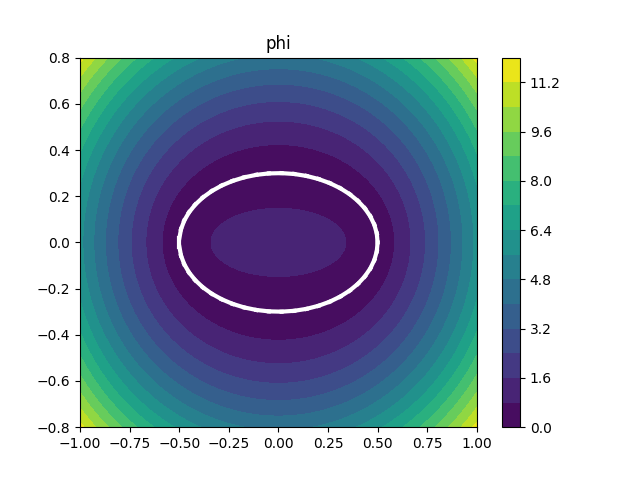
\includegraphics[width=0.7\linewidth]{"article/REQ_ellipse.png"}
		\caption{ADF par REQ sur une ellipse.}
		\label{REQ}
	\end{figure}
\end{minipage}
\begin{minipage}{0.58\linewidth}
	\begin{figure}[H]
		\centering
		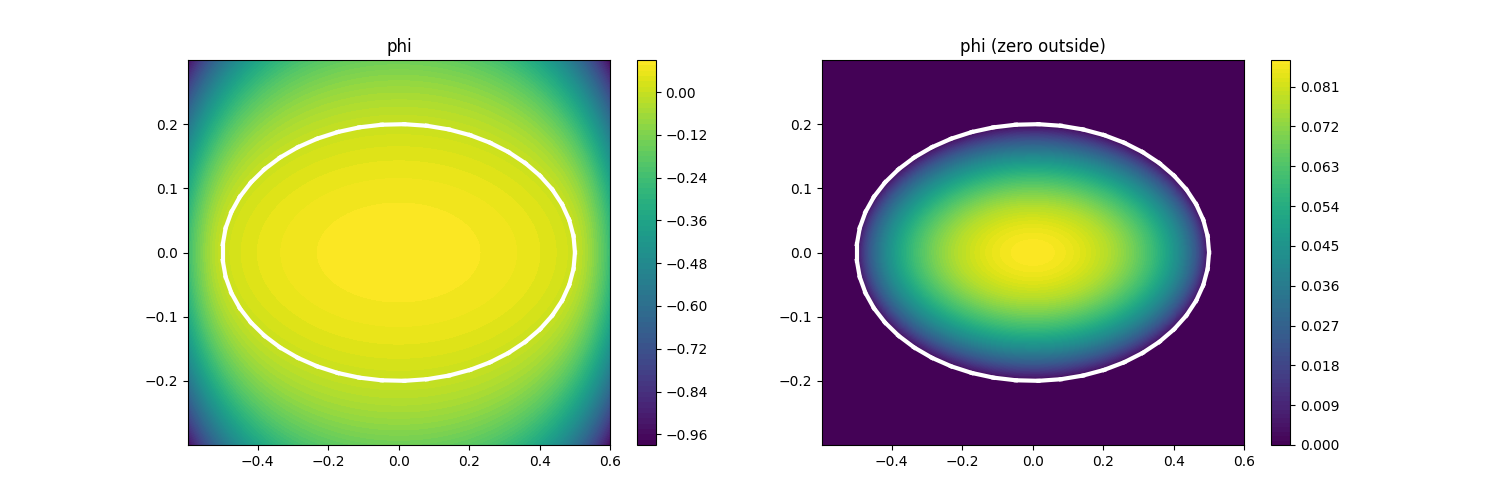
\includegraphics[width=\linewidth]{"article/MVP_ellipse.png"}
		\caption{ADF par MVP sur une ellipse.}
		\label{MVP}
	\end{figure}
\end{minipage}

\subsection{Entraînement du PINNs à apprendre une solution unique}

\subsubsection{Problème considéré}

\textbf{EDP :} On considère le problème de Poisson avec condition de Dirichlet homogène ($g=0$), définie par

Trouver $u : \Omega \rightarrow \mathbb{R}^d (d=1,2,3)$ tel que
\begin{equation}
	\left\{
	\begin{aligned}
		-\Delta u &= f, \; &&\text{dans } \; \Omega, \\
		u&=g, \; &&\text{sur } \; \partial\Omega,
	\end{aligned}
	\right. \tag{$\mathcal{P}$} \label{pb_initial}
\end{equation}
avec $\Delta$ l'opérateur de Laplace.

\textbf{Géométrie :} On considère $\Omega$ comme étant un cercle de rayon $r$ et de centre $(x_0,y_0)$. 

Pour simplifier, on va considérer que $\Omega$ est entièrement contenu dans un carré $\mathcal{O}$ (Figure \ref{geom_circle}). 

\begin{minipage}{0.38\linewidth}
	\begin{figure}[H]
		\centering
		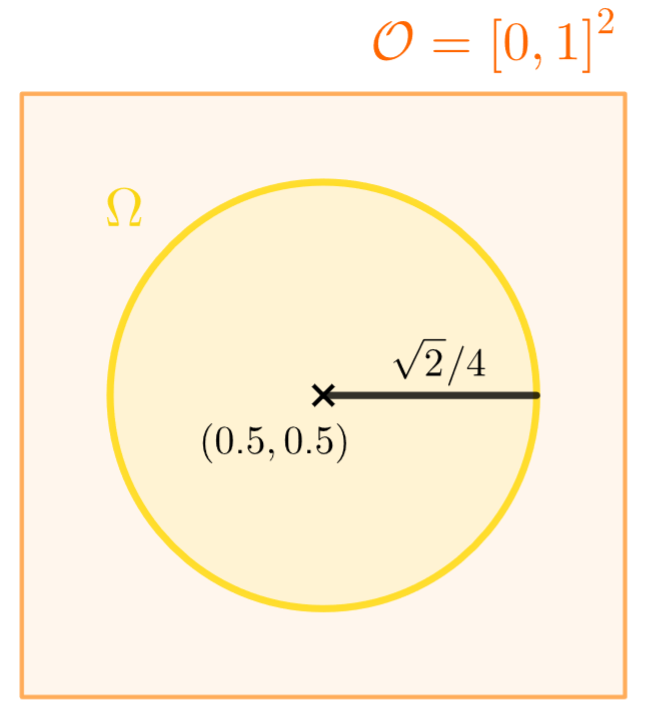
\includegraphics[width=0.7\linewidth]{"training/geom_circle.png"}
		\caption{Domaine considéré.}
		\label{geom_circle}
	\end{figure}
\end{minipage}
\begin{minipage}{0.68\linewidth}
	On considère la solution analytique $u_{ex}$, définie par
	\begin{equation*}
		u_{ex}(x,y)=S\times\sin\left(\frac{1}{r^2}\pi((x-x_0)^2+(y-y_0)^2)\right)
	\end{equation*}
	
	Ce qui nous fournit le terme source $f$, définie par
	\begin{align*}
		f(x,y)=\frac{4}{r^4}\pi^2&S((x-x_0)^2+(y-y_0)^2)\sin\left(\frac{1}{r^2}\pi((x-x_0)^2+(y-y_0)^2)\right) \\
		&-\frac{4}{r^2}\pi S \cos\left(\frac{1}{r^2}\pi((x-x_0)^2+(y-y_0)^2)\right)
	\end{align*}
\end{minipage}
\begin{Rem}
	On voit que sur le cercle, le problème est bien homogène.
	
	De plus, on notera qu'un choix simple peut être de prendre le carré $[x_0-r-\epsilon,x_0+r+\epsilon]\times[y_0-r-\epsilon,y_0+r+\epsilon]$ où $\epsilon>0$ est un paramètre fixé dans le but que $\Omega$ soit entièrement compris dans $\mathcal{O}$.
\end{Rem}

\subsubsection{Entraînement du PINNs}

On fixe $r=\sqrt{2}/4$, $(x_0,y_0)=(0.5,0.5)$ et $S=0.5$ et on considère ici que l'on souhaite entraîner un PINNs à apprendre cette solution. On utilisera l'implémentation développé dans le module ScimBA\footnote{\url{https://sciml.gitlabpages.inria.fr/scimba/}}. 

On notera que l'article 2104.08426 présente comment imposer les conditions au bord de manière exacte. C'est pourquoi, on considérera deux cas :
\begin{enumerate}[label=\textbullet]
	\item on apprend directement la solution $u$. La loss totale regroupe alors la loss sur le résidu et la loss sur le bord.
	\item on apprend $w$ tel que $u=\phi w$ avec $\phi$ notre fonction levelset. La loss ne contient alors que la loss sur le résidu. 
\end{enumerate}
Ainsi, une première étape a été de rajouter, dans l'implémentation de ScimBa, la possibilité de définir un domaine à partir d'une fonction levelset. Ainsi pour obtenir un sampling de points à l'intérieur de $\Omega$, il suffit de générer un échantillon de point sur le carré $\mathcal{O}$ et de ne garder que les points tels que $\phi(x,y)<0$. Pour générer un échantillon de point sur le bord du domaine $\Omega$, on a fait le choix pour l'instant de prendre les points tels que $|\phi(x,y)|<\epsilon$ avec $\epsilon=1e-5$ (Figure \ref{sampling_0}).

\begin{figure}[H]
	\centering
	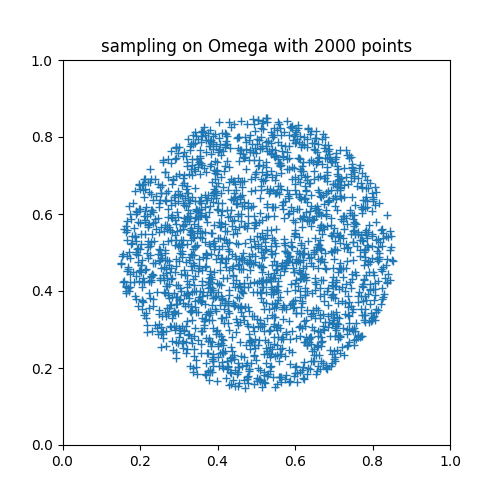
\includegraphics[width=0.5\linewidth]{"training/sampling_0.png"}
	\caption{Sampling à l'intérieur et au bord du cercle considéré.}
	\label{sampling_0}
\end{figure}

\begin{Rem}
	Pour le sampling du bord, c'est un choix qui ne sera pas conserver, il faudra trouver une solution plus rapide-précise que celle-ci.
\end{Rem}

On peut alors entraîner le PINNs à apprendre notre solution. On choisira la configuration suivante :
\begin{figure}[H]
	\centering
	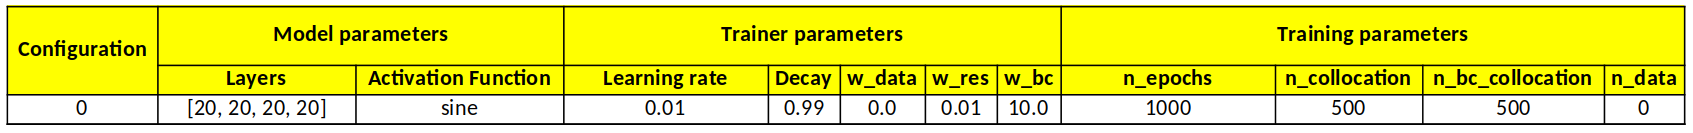
\includegraphics[width=\linewidth]{"training/config_0.png"}
	\caption{Paramètres d'entraînement considéré pour le PINNs.}
	\label{config_0}
\end{figure}

On va alors entraîner un modèle à apprendre $u$ (Figure \ref{model_0}) et un autre à apprendre $w$ (Figure \ref{model_0_exact_bc}) avec ces mêmes paramètres dans le but de comparer les résultats.

\begin{minipage}{0.48\linewidth}
	\begin{figure}[H]
		\centering
		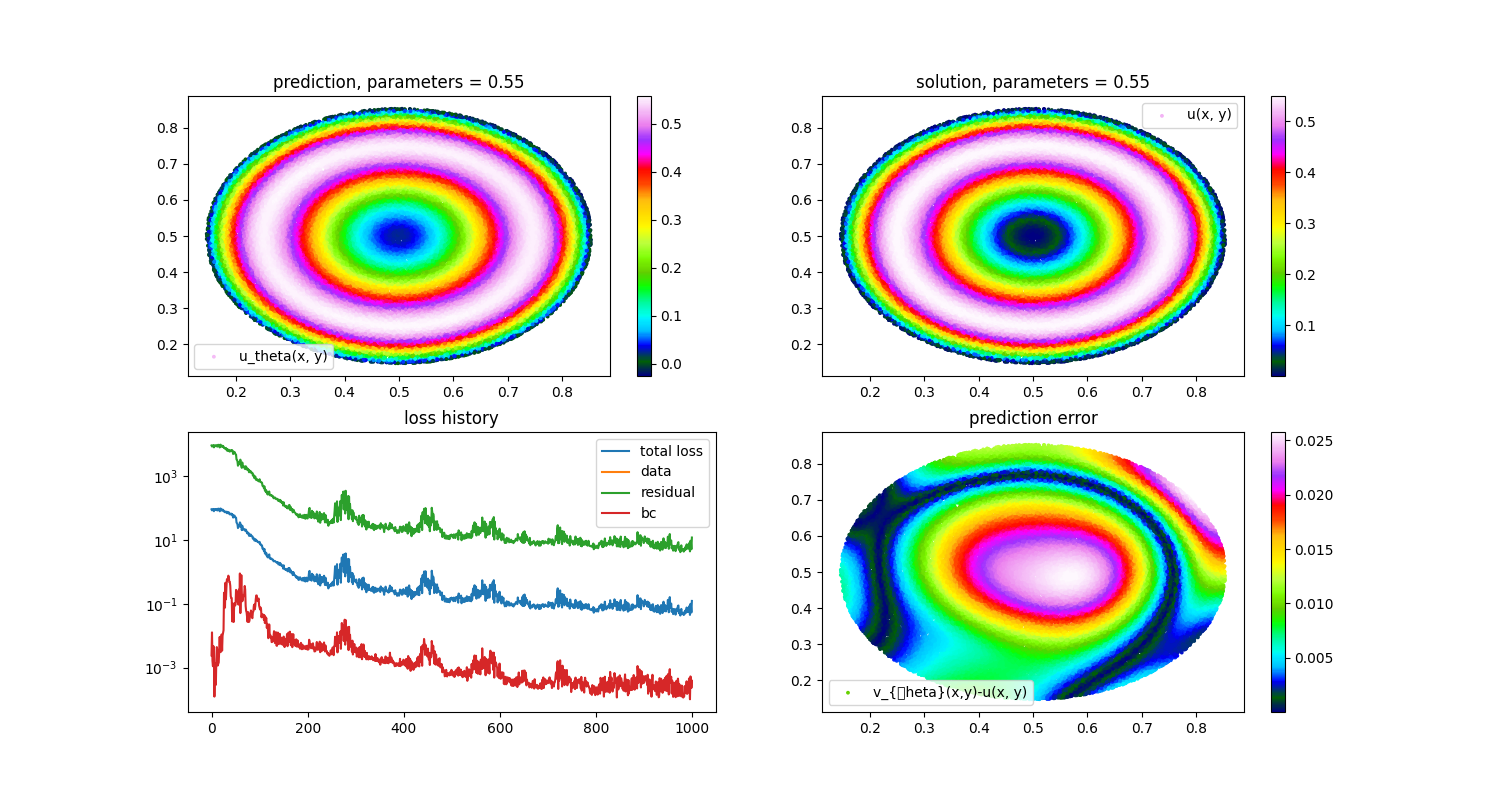
\includegraphics[width=\linewidth]{"training/model_0.png"}
		\caption{Fin d'entraînement - Modèle sur $u$.}
		\label{model_0}
	\end{figure}
\end{minipage}
\begin{minipage}{0.48\linewidth}
	\begin{figure}[H]
		\centering
		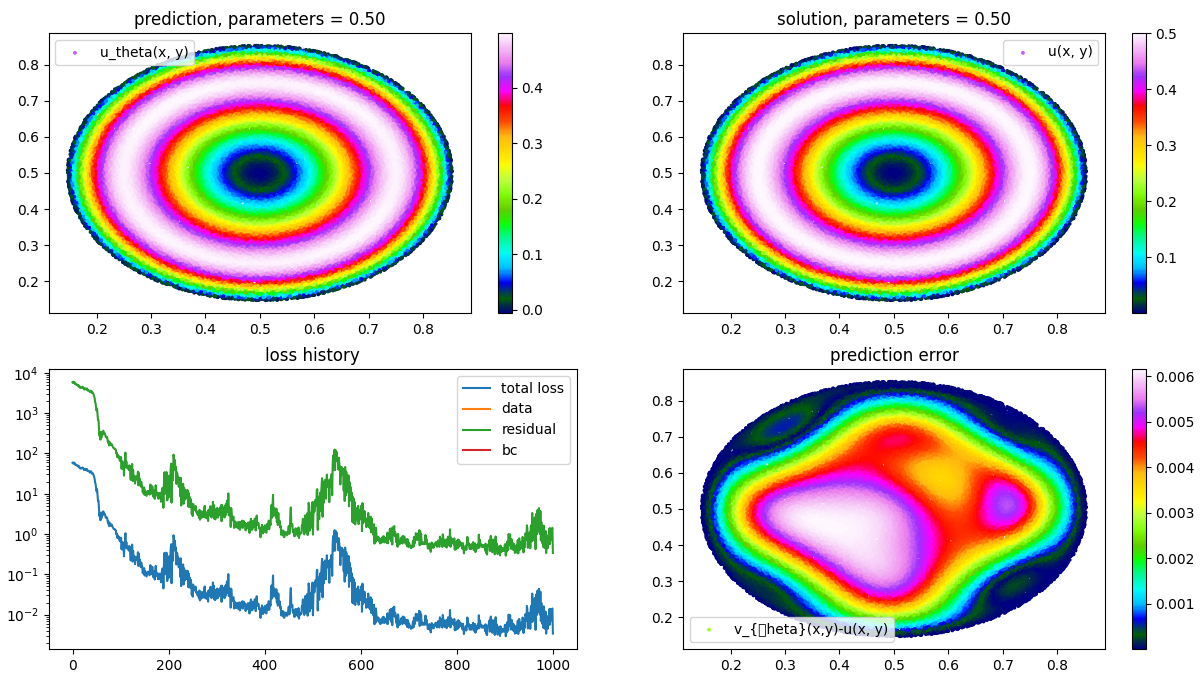
\includegraphics[width=\linewidth]{"training/model_0_exact_bc.png"}
		\caption{Fin d'entraînement - Modèle sur $w$.}
		\label{model_0_exact_bc}
	\end{figure}
\end{minipage}

\begin{Rem}
	Il semblerait que le modèle sur $w$ soit 10 fois plus précis en terme d'erreur.
	
	De plus, on remarque bien, sur la carte d'erreur, sur le modèle sur $u$ a des erreurs au bord, ce qui risque de poser problème dans la correction. 
\end{Rem}

\subsubsection{Correction sur les prédictions du PINNs}

On note $\tilde{\phi}$ la prédiction d'un des PINNs précédent. On ne va considérer ici que la correction par addition, on pose alors
\begin{equation*}
	\tilde{u}=\tilde{\phi}+\tilde{C}
\end{equation*}
et on cherche à trouver $\tilde{C}: \Omega \rightarrow \mathbb{R}^d$ solution du problème
\begin{equation*}
	\left\{\begin{aligned}
		-\Delta \tilde{u}&=f, \; &&\text{on } \Omega, \\
		\tilde{u}&=g, \; &&\text{in } \Gamma.
	\end{aligned}\right.
\end{equation*}
avec $g=0$ dans le cas considéré.
On cherche alors à trouver $\tilde{C}: \Omega \rightarrow \mathbb{R}^d$ solution du problème
\begin{equation*}
	\left\{\begin{aligned}
		-\Delta \tilde{C}&=\tilde{f}, \; &&\text{on } \Omega, \\
		\tilde{C}&=0, \; &&\text{in } \Gamma.
	\end{aligned}\right. %\tag{$\mathcal{C}_{+}$}
\end{equation*}
avec $\tilde{f}=f+\Delta\tilde{\phi}$.

On cherche alors à tester la correction sur les deux modèles précédents (celui où on apprend $u$ et celui où on apprend $w$). On testera l'utilisation de FEM et de $\phi$-FEM dans les deux cas.

\textbf{Résultats avec le modèle sur $u$ :}

\begin{minipage}{0.48\linewidth}
	\begin{figure}[H]
		\centering
		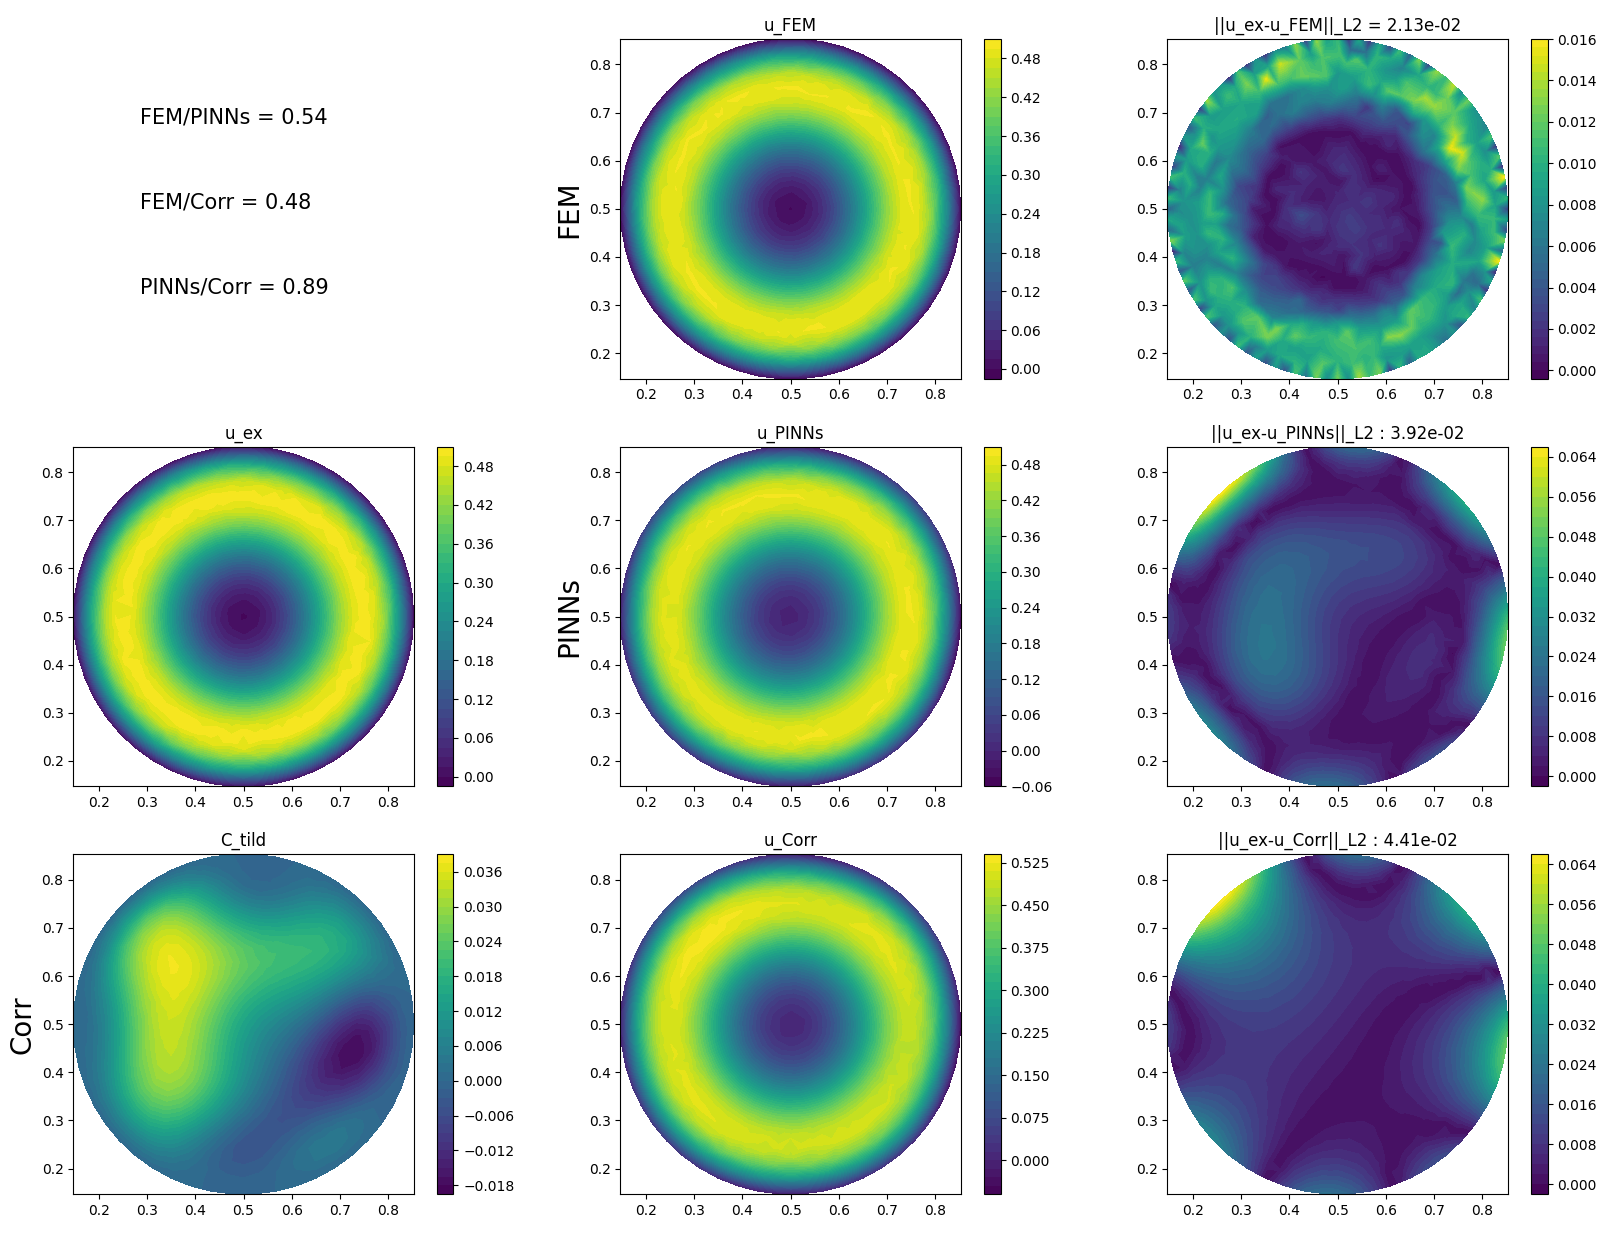
\includegraphics[width=\linewidth]{"corr/corr_fem_0.png"}
		\caption{Correction avec FEM - Modèle sur $u$.}
		\label{corr_fem_0}
	\end{figure}
\end{minipage}
\begin{minipage}{0.48\linewidth}
	\begin{figure}[H]
		\centering
		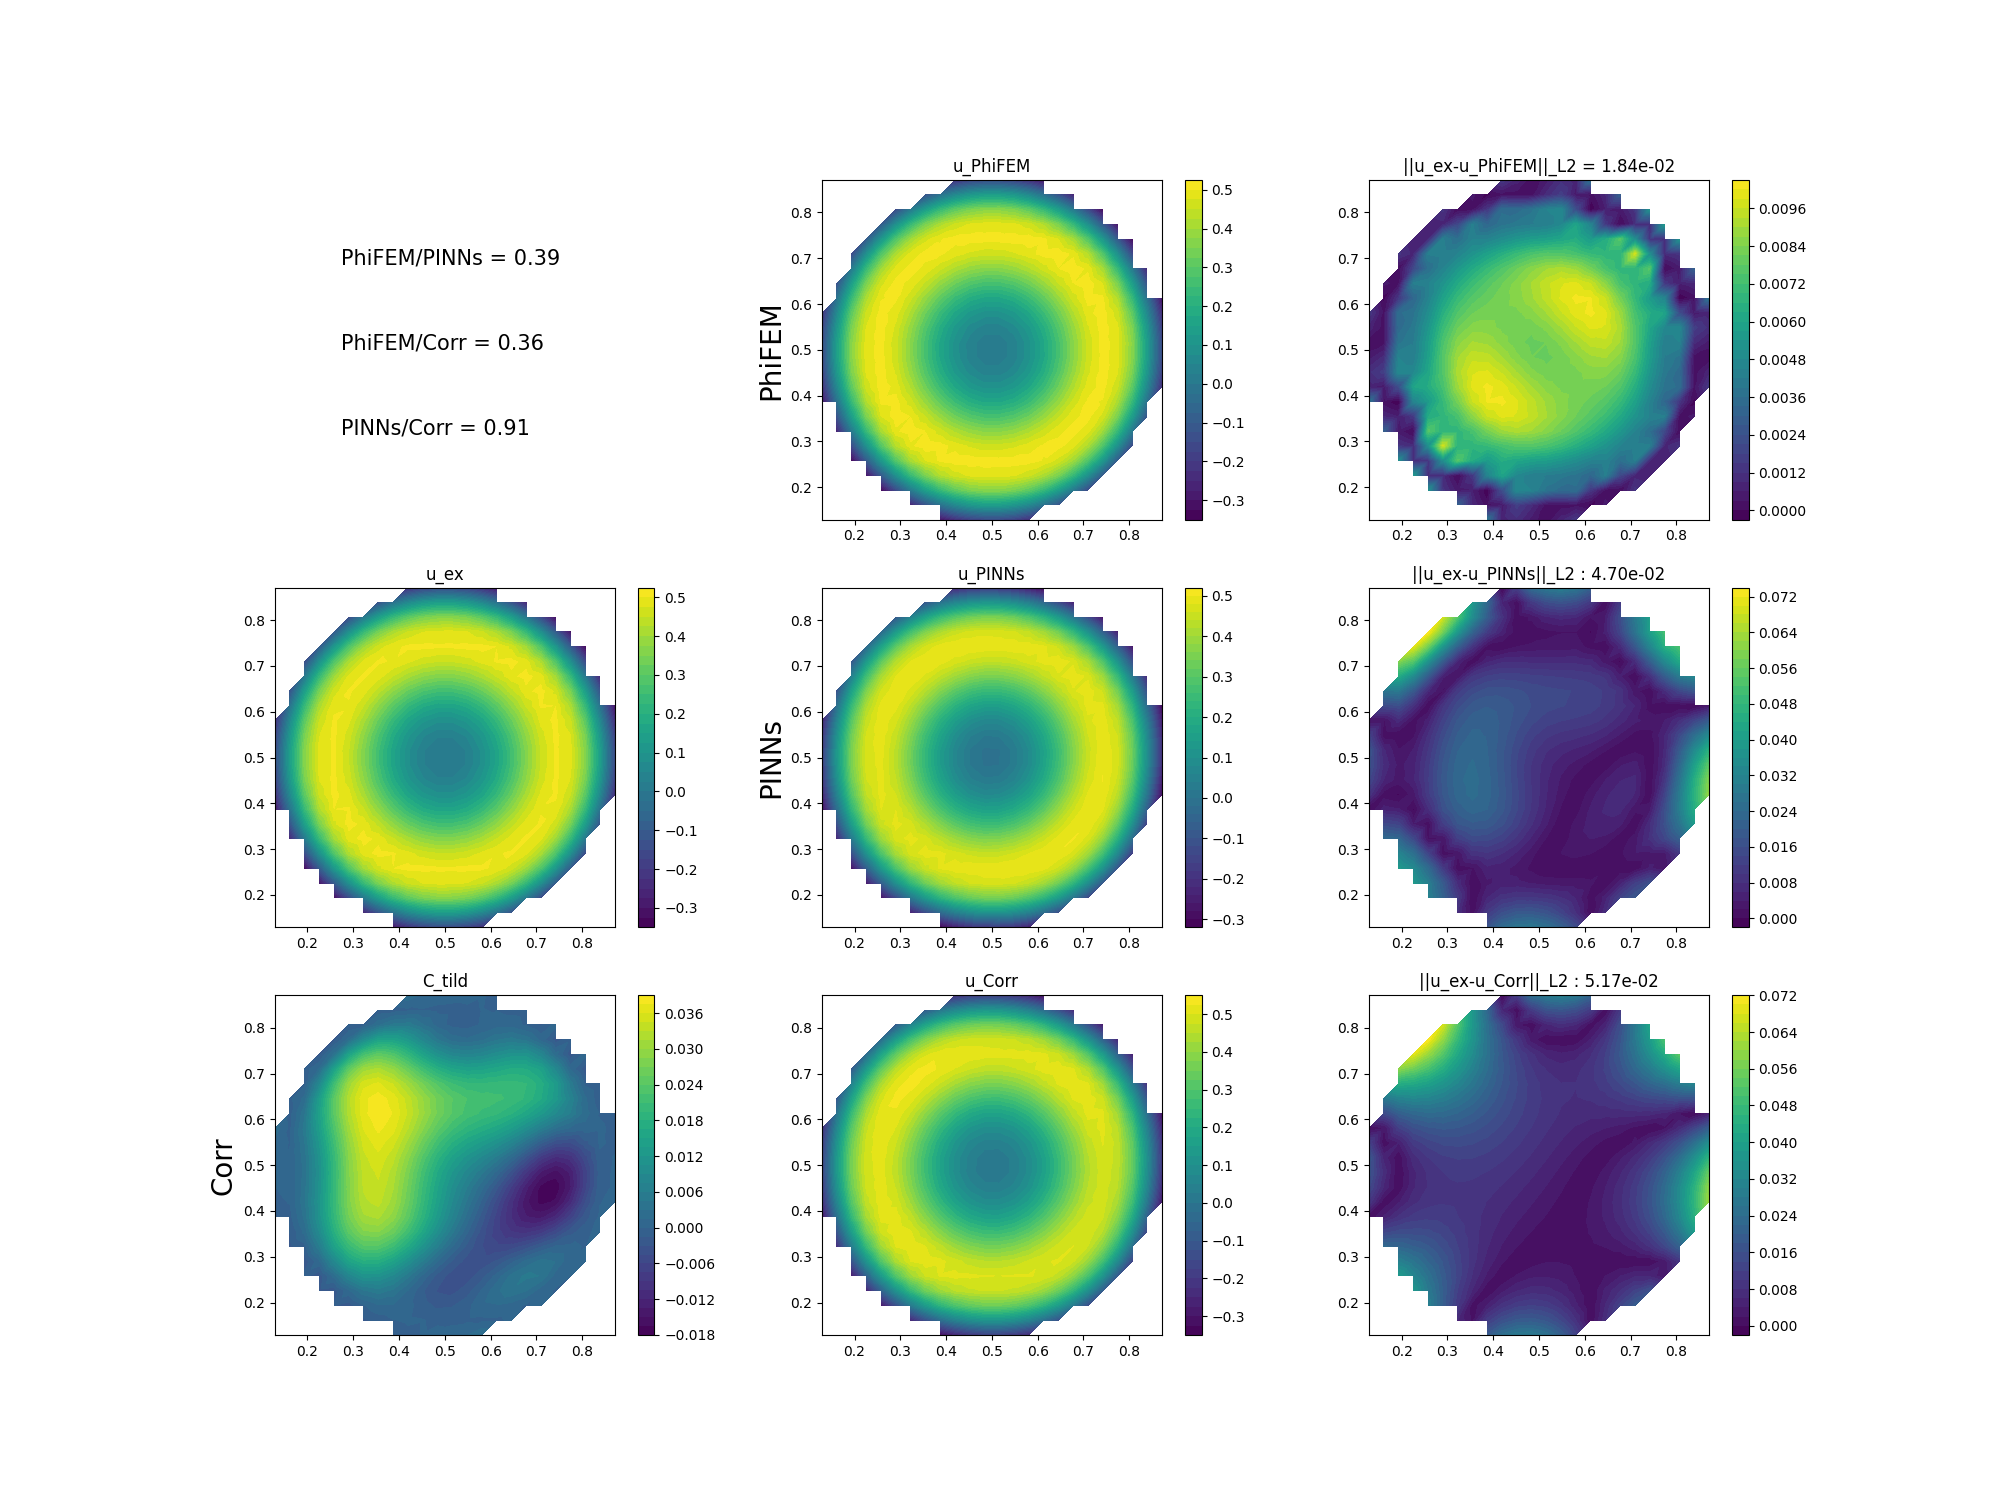
\includegraphics[width=\linewidth]{"corr/corr_phifem_0.png"}
		\caption{Correction avec $\phi$-FEM - Modèle sur $u$.}
		\label{corr_phifem_0}
	\end{figure}
\end{minipage}

\textbf{Résultats avec le modèle sur $w$ :}

\begin{minipage}{0.48\linewidth}
	\begin{figure}[H]
		\centering
		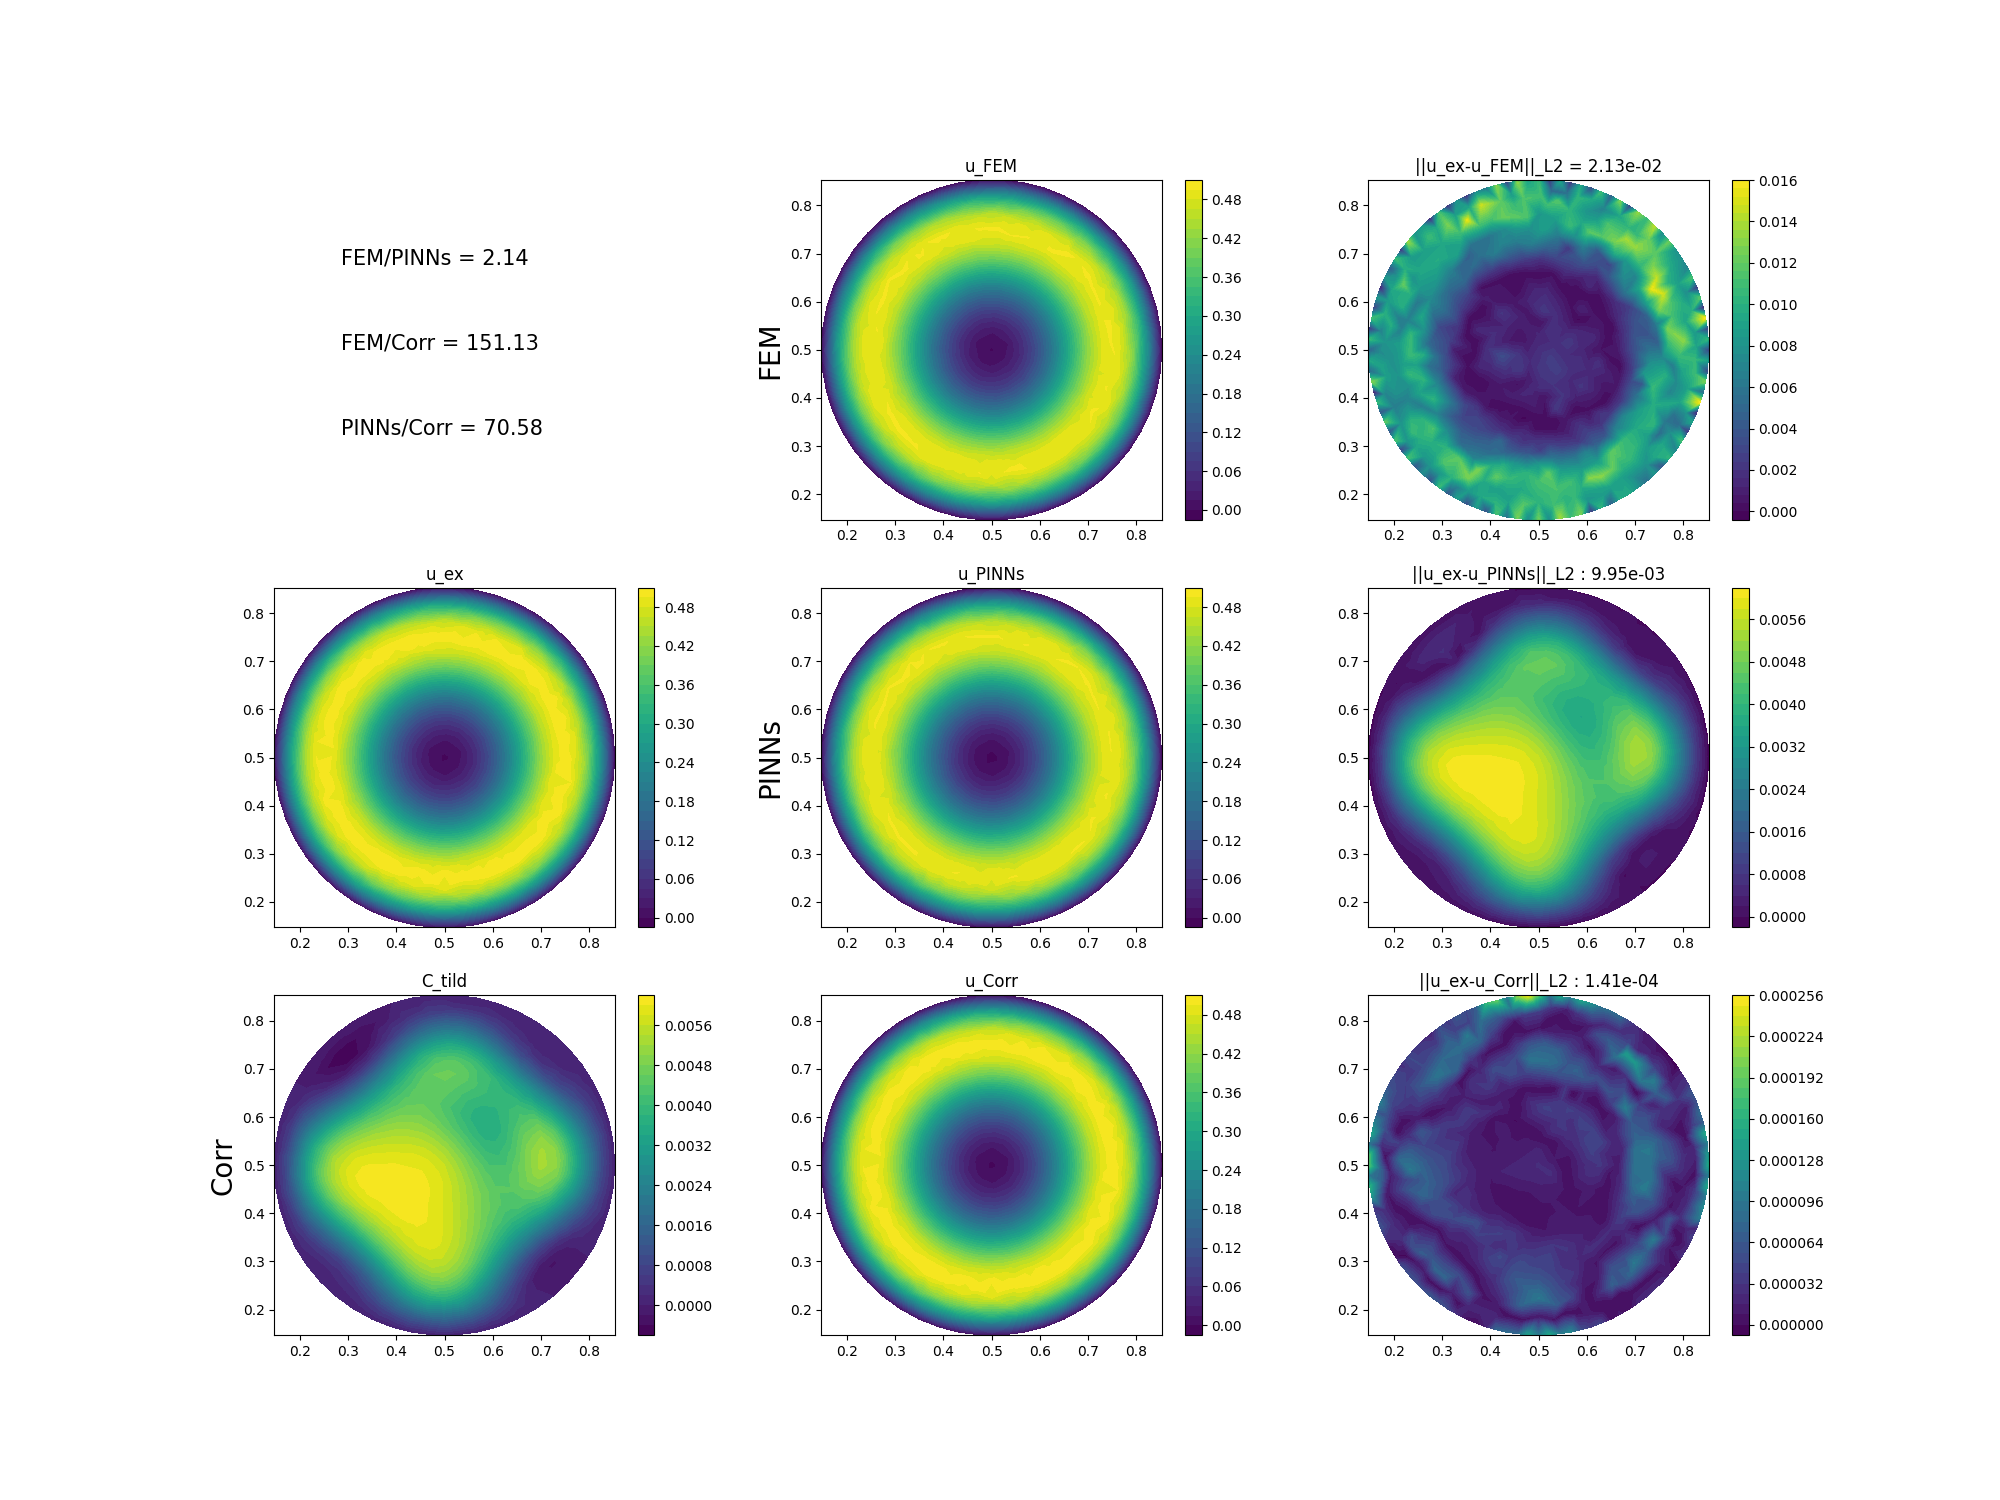
\includegraphics[width=\linewidth]{"corr/corr_fem_0_exact_bc.png"}
		\caption{Correction avec FEM - Modèle sur $w$.}
		\label{corr_fem_0_exact_bc}
	\end{figure}
\end{minipage}
\begin{minipage}{0.48\linewidth}
	\begin{figure}[H]
		\centering
		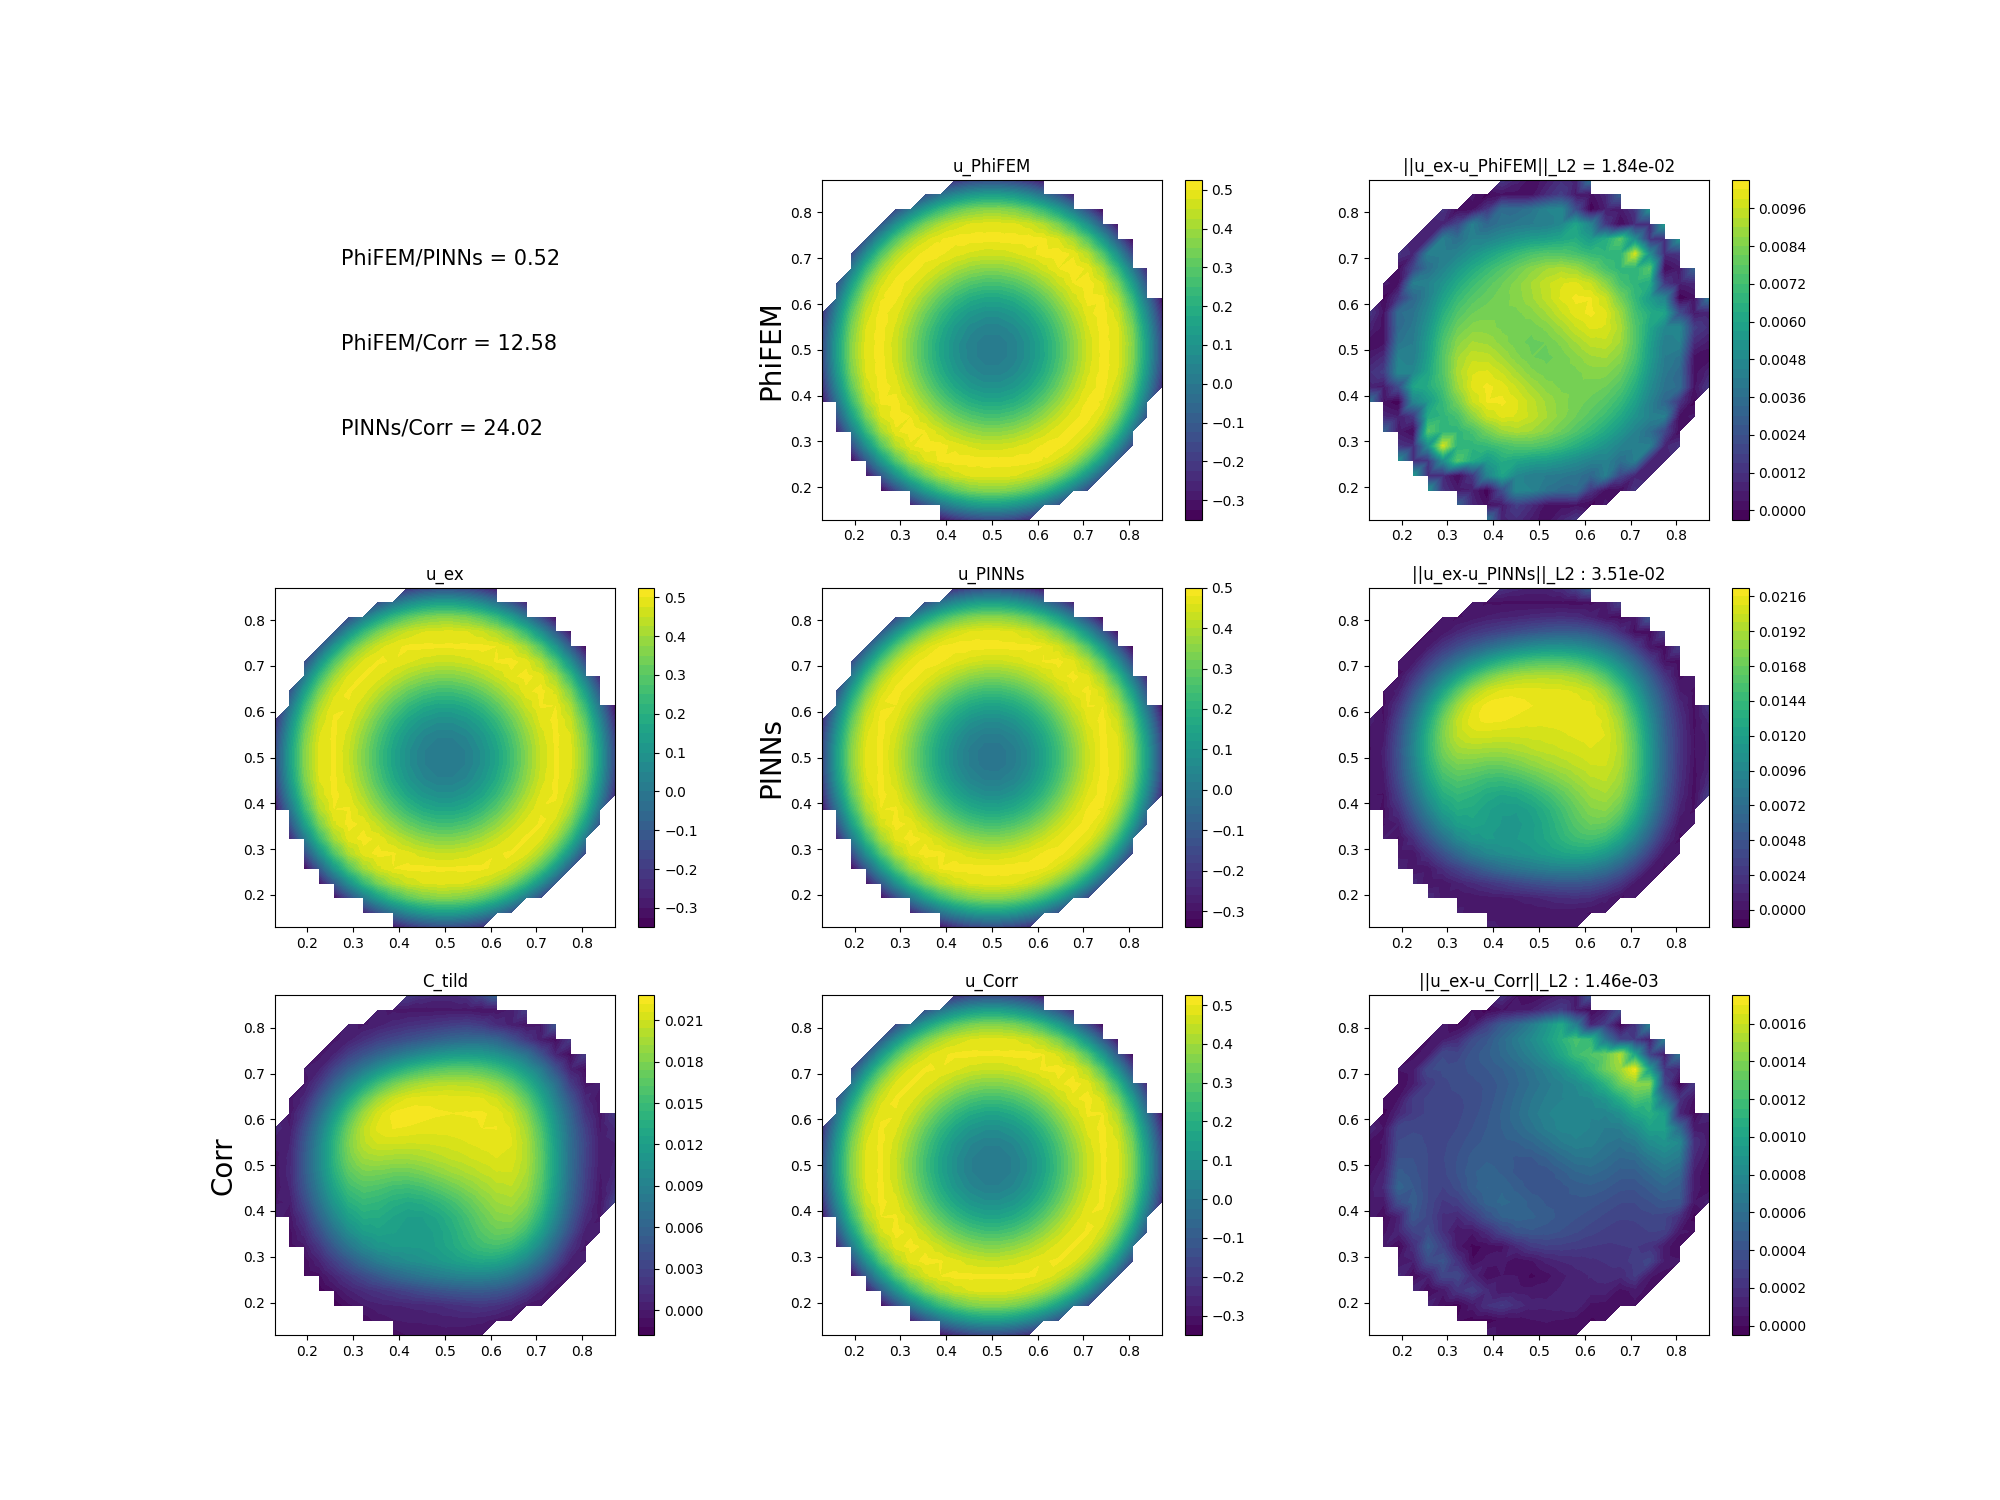
\includegraphics[width=\linewidth]{"corr/corr_phifem_0_exact_bc.png"}
		\caption{Correction avec $\phi$-FEM - Modèle sur $w$.}
		\label{corr_phifem_0_exact_bc}
	\end{figure}
\end{minipage}

	\section{Week 5 : 30/10/2023 - 03/11/2023}
	(ABSENTE du Lundi au Mercredi car Malade)

\textbf{Réunions :}
\begin{enumerate}[label=\textbullet]
	\item \textit{Lundi après-midi} - Réunion (Michel + Vanessa) $\rightarrow$ ABSENTE (MALADE)
	\item \textit{Mardi matin} - Réunion d'équipe - ? $\rightarrow$ ABSENTE (MALADE)
	\item \textit{Vendredi matin} - TP d'Informatique L2S3 $\rightarrow$ NON (Vacance scolaire)
	\item \textit{Vendredi après-midi} - Réunion (Michel)
\end{enumerate}
\textbf{Fait durant la semaine :}
\begin{enumerate}[label=\textbullet]
	\item Lecture de l'article 2301.05187 (WIRE)
	\item Bibliographie (recherche de papier sur les INR)
	\item Projection des solutions $\phi$-FEM sur $\Omega$ pour le calcul des erreurs
\end{enumerate}

\textbf{A faire :}
\begin{enumerate}[label=\textbullet]
	\item Lire nouvel article 2006.09661 ("Implicit Neural Representations with Periodic Activation Functions")
	\item Préparer document résultats $\rightarrow$ réunion Lundi 06/11/2023
\end{enumerate}

	\section{Week 6 : 06/11/2023 - 10/11/2023}
\end{document}